\chapter{Análisis y Desarrollo del Diseño del Sistema Interactivo}

El diseño propuesto es elaborado a partir de los requerimientos recopilados por parte del cliente y Product Owner (ya que tanto el cliente como el rol es asignado a la misma persona).

El objetivo de la propuesta es satisfacer las necesidades del usuario que emplee el resultado de la investigación e implementación de este sistema interactivo. La propuesta será diseñada a partir de las bases de la ingeniería de Requerimientos aplicada en la metodología ágil SCRUM.

La Ingeniería de requerimientos del proyecto implica establecer lo que el cliente y usuario requiere del sistema interactivo \cite{scrumdiapo}, además de la funcionalidad esperada del proyecto, se debe definir, especificar y validar los requerimientos para poder aprobar su elaboración.

De la siguiente manera la solicitud del cliente inicia con un pedido ambiguo y coloquial por parte del instructor de artes marciales de uno de los integrantes del grupo al compartir su idea con el, juntos anotaron sus pensamientos con las siguientes palabras: "Me gustaría un juego con el cual pueda entrenar las poses y técnicas básicas de Karate siguiendo lo que hace en la pantalla y que me diga si lo hago bien o mal, pero no tengo un Kinect o una consola para jugar, solo mi laptop", a lo cual el estudiante añadió "Pero también sería genial que puedas bailar e imitar lo que hace la gente, si va por esa línea, podrías generalizarlo para atraer más público". Es de conocimiento general que las ideas suelen venir de lugares inesperados, en este caso, fue una conversación coloquial entre dos conocidos lo que inspiro el proyecto, a partir de esas palabras, se determina la base del proyecto, por tanto, se debe recabar entre las frases, se las dividirá e interpretará dividiéndolo en 4 secciones como se ven en la tabla \ref{requerimientos}. Si bien, el instructor perdió el interés en el proyecto con el pasar del tiempo, el estudiante tomará el rol de cliente para el desarrollo del sistema interactivo.


\begin{table}[t]
	\begin{center}
		\begin{tabular}{|m{7cm}|m{8cm}|}
			\hline Solicitud en lenguaje coloquial & Interpretación inicial como requerimiento \\ \hline
			\multirow{3}{7cm}{Me gustaría un juego con el cual pueda entrenar las poses y técnicas básicas de Karate siguiendo lo que hace en la pantalla.}
			& Desarrollar un sistema interactivo.\\ 
			& Existe un vídeo o instrucción en una pantalla para poder entrenar artes marciales.\\ & El usuario debe moverse acorde lo visto en la pantalla. \\ \hline
			Que me diga si lo hago bien o mal. & Se requiere de un sistema de calificaciones para los movimientos hechos por el usuario. \\ \hline
			No tengo un Kinect o una consola para jugar, solo mi laptop. & Tiene que funcionar en una laptop. \\ \hline
			Sería genial que puedas bailar e imitar lo que hace la gente. & No debe limitarse a artes marciales. \\ \hline
		\end{tabular}
		\caption{Interpretación de la solicitud inicial del cliente}
		\label{requerimientos}
		\footnotesize Fuente: Elaboración Propia.
	\end{center}
\end{table}

Posteriormente, se vio conveniente ser capaz de usar vídeos proporcionados por el usuario para poder crear niveles propios, ya que si inicialmente el instructor lo deseaba para entrenar poses y técnicas de Karate, él habría provisto de los vídeos, sin embargo, se emplearan recursos de terceros para realizar las pruebas del prototipo que se desarrolle.

\section{Análisis de Requerimientos}

En un principio, se debe definir como se llamará a los distintos vídeos que se desean imitar, formalmente se lo conocerá en el contexto como: \textbf{Mapa, mapa es un conjunto de poses que el usuario debe imitar en tiempo cronometrado de un determinado vídeo}. 

Se desarrolla un sistema interactivo que permite al usuario poder jugar distintos mapas y además crear mapas propios, para ello se requieren dos funciones fundamentales.

\begin{itemize}
	\item Play: Refiere al acto de entrar a una lista de mapas de usuario, donde se seleccionará un mapa y se realizará el seguimiento de las acciones provistas por el sistema interactivo a imitar.	
	\item Crear un nuevo mapa: Término dado a la elaboración de mapas, donde el usuario provee un vídeo que quiera convertir en un mapa del sistema interactivo.
\end{itemize}

Se debe dar a conocer la forma en que los usuarios interactúan con el sistema interactivo, definir ciertas limitación, realizar consideraciones respecto a la interfaz gráfica y a las modificaciones externas del producto.

\subsubsection{Características de Usuario}

El sistema interactivo contará con una categoría Apto para todo público según el sistema PEGI y Early Childhood en el sistema ESRB, por tanto los usuarios puede ser cualquier persona mayor a los 3 años que pueda emplear el sistema interactivo. Sin embargo, debido a que esta diseñado para realizar actividad física, se recomienda un control de salud previo uso para no resultar herido o lastimado en caso de ser mayor de edad o tener problemas que limiten las actividades físicas.
La creación de los mapas requiere de la lectura de un ligero manual de usuario y perseverancia para la actividad tediosa, por tanto, si bien puede hacerlo cualquiera, es recomendado que lo hagan mayores de 12 años.


\subsection{Requerimientos Funcionales}

Los requerimientos funcionales hacen referencia a todas las funcionas que tiene disponible el usuario para realizar dentro del sistema interactivo, según los módulos y componentes externos que lo integran. Se mencionaron dos requerimientos funcionales, los cuales, se descomponen en:

\subsubsection{Play}

\begin{enumerate}
	\item Jugar: La opción de afirmar que se jugara, debe dirigirte a seleccionar el mapa deseado.
	\item Opciones: El usuario es capaz de interactuar con las opciones descritas en 3 y 4.
	\item Subir/Bajar el volumen: Una de las opciones es poder subir y bajar el volumen del audio del vídeo en una escala de 0 a 1.
	\item Cambiar la resolución: Una opción más, esta permitirá el cambio del tamaño de la ventana del sistema interactivo, debe tener múltiples resoluciones disponibles.
	\item Seleccionar el nivel deseado: Una vez se elije jugar, el usuario puede seleccionar el mapa con el que interactuar.
	\item Salir: La opción de dejar de ejecutar el sistema interactivo.
	\item Mostrar calificación al terminar el mapa: Un usuario debe ser capaz de visualizar la calificación que va acumulando a medida que realiza el nivel.
	\item Salir del mapa: La capacidad del usuario para interrumpir el seguimiento del mapa.
	\item Pausar juego: El usuario debe ser capaz de detener el mapa en proceso cuando este haya sido selecto para ejecutar.
\end{enumerate}

\subsubsection{Crear un nuevo mapa}

Para la creación de un mapa, se tiene que seguir una serie de 5 pasos que involucran al usuario:

\begin{enumerate}
	\item Ejecutar Script de conversión de vídeo a JSON e imágenes en formato JPG: El usuario selecciona un vídeo, usará un Script para el primer paso de conversión a un mapa.
	\item Ejecutar Script de JSON a .txt: Posteriormente, se vuelve a usar otro Script para una segunda conversión a un formato intuitivo de entender para el usuario
	\item Selección manual de poses: Para crear un mapa, solo se requieren poses específicas para cada movimiento, se borran las que se consideren redundantes de entre los txt.
	\item Guardar el resultado en una carpeta designada para los mapas del usuario: Se guarda en una carpeta el nuevo mapa, en preparación al siguiente paso.
	\item Añadir un margen de tiempo para realizar las poses: Todas las poses de cada nivel tienen que tener una variable que determine el tiempo límite que se tiene para realizar esa acción. 
\end{enumerate}

\subsection{Requerimientos No Funcionales}

Los requerimientos no funcionales indican los limites del sistema o el proceso de desarrollo, entre ellos se emplearan:

\begin{enumerate}
	\item Interfaz Gráfica de Usuario: Desarrollar una interfaz de usuario, para poder emplear fácilmente los requerimientos funcionales,el sistema interactivo de una manera más efectiva.
	\item Funcionalidad: Que la capacidad del sistema interactivo sea capaz de funcionar acorde lo mencionado en los requerimientos funcionales.
	\item Confiabilidad: Inicialmente, el plug-in de Unity tiene una tendencia a cerrarse repentinamente y al abrirlo por primera vez viene con archivo corruptos que se tienen que arreglar, se espera solucionar o al menos reparar esta debilidad de ser posible.
	\item Intuitividad: Se espera que el cliente sea capaz de entender que actividad hacer con solo ver las funciones disponibles en la interfaz gráfica.
\end{enumerate}
\newpage
\subsection{Funcionalidad Esperada del Sistema Interactivo}

Se prepara un resumen visual de los requerimientos solicitados por el cliente, donde se separan los dos tipos de usuario que emplearán el producto final

\begin{figure}[h]
	\centering
	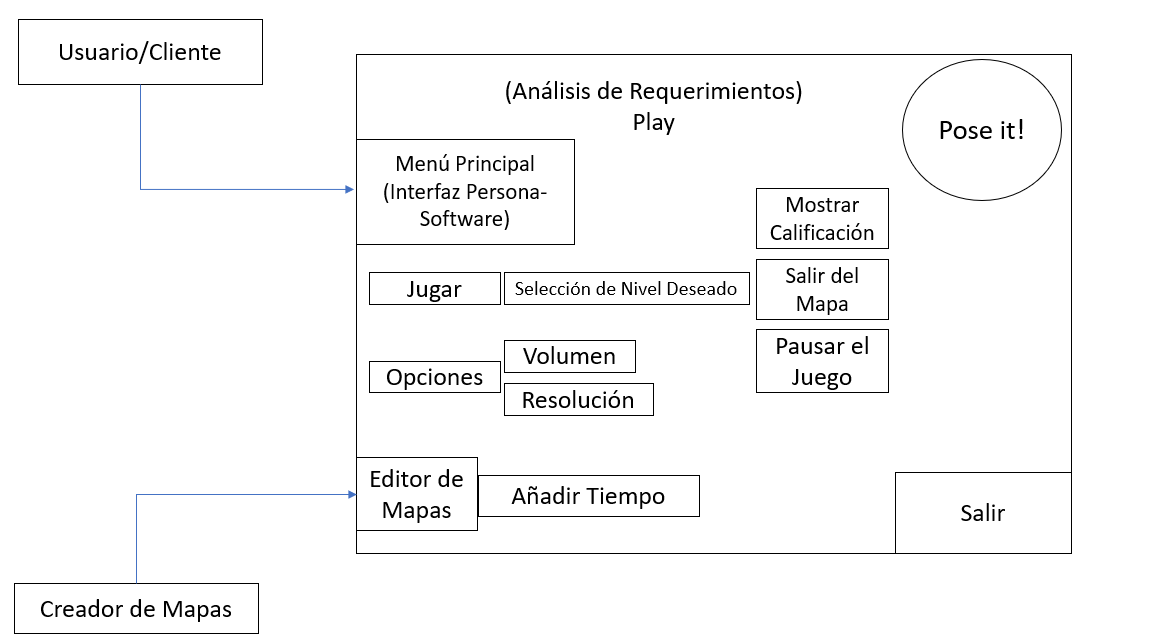
\includegraphics[width=16cm,height=10cm,]{./Images/requerimientosgraficaposeit.png}
	\caption{Ilustración de Requerimientos en la GUI}
	\footnotesize Fuente: Elaboración Propia
	\label{requerimientosgrafico}
\end{figure}

\newpage
\subsection{Diagrama de Flujo de Datos}


\begin{figure}[h]
\centering
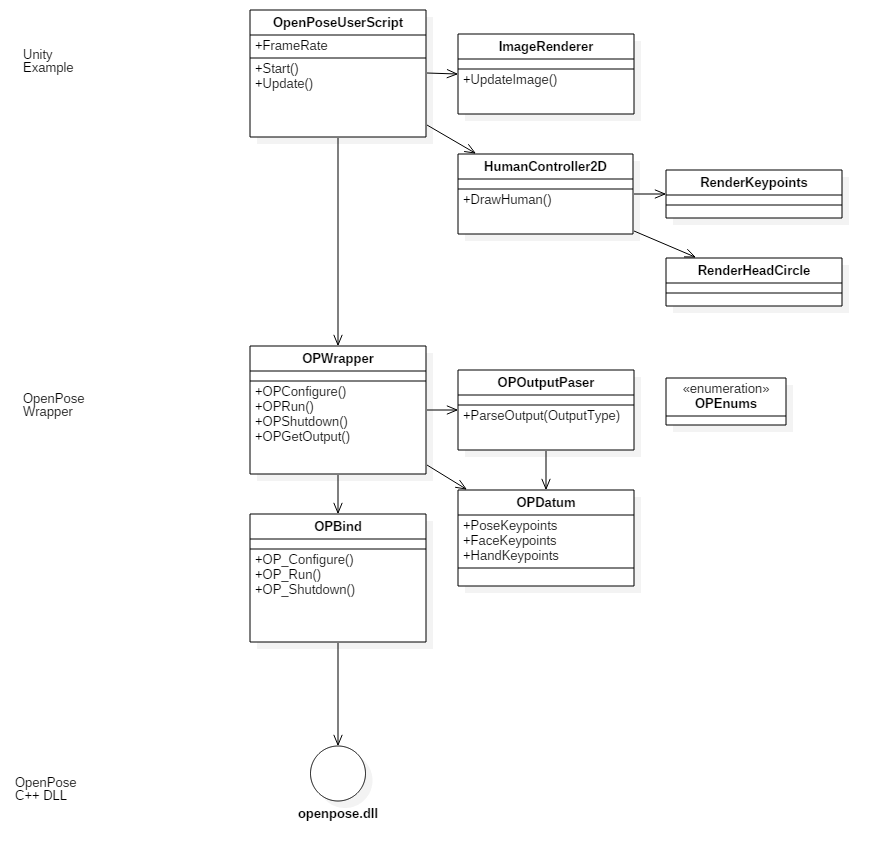
\includegraphics[width=14cm,height=15cm,]{./Images/futurediagramaderequisitos.png}
\caption{Diagrama de Datos de Flujo}
\footnotesize Fuente: Modificación de la versión original del plug-in de OpenPose\cite{8765346}
\label{dfd}
\end{figure}


